\section{Technical Implementation}
\label{section:techimpl}
This section describes the current solution, the implemented software architecture and the final results of the project.
Discrepancies between the planned implementation approach and the current solution are listed in \sectionref{section:techimpl:comparison_impl}.

\subsection{System Overview}
The following graphics displays the current system overview.
As described in \sectionref{section:techimpl:arcgis} and \sectionref{section:project:swisstoporeplacement}, instead of the elevation model data from \emph{swisstopo}, a Unity plugin for \emph{ArcGIS} maps services was used.
This change is reflected in the new system overview, and is the only adjustment that was made.

\begin{figure}[H]
    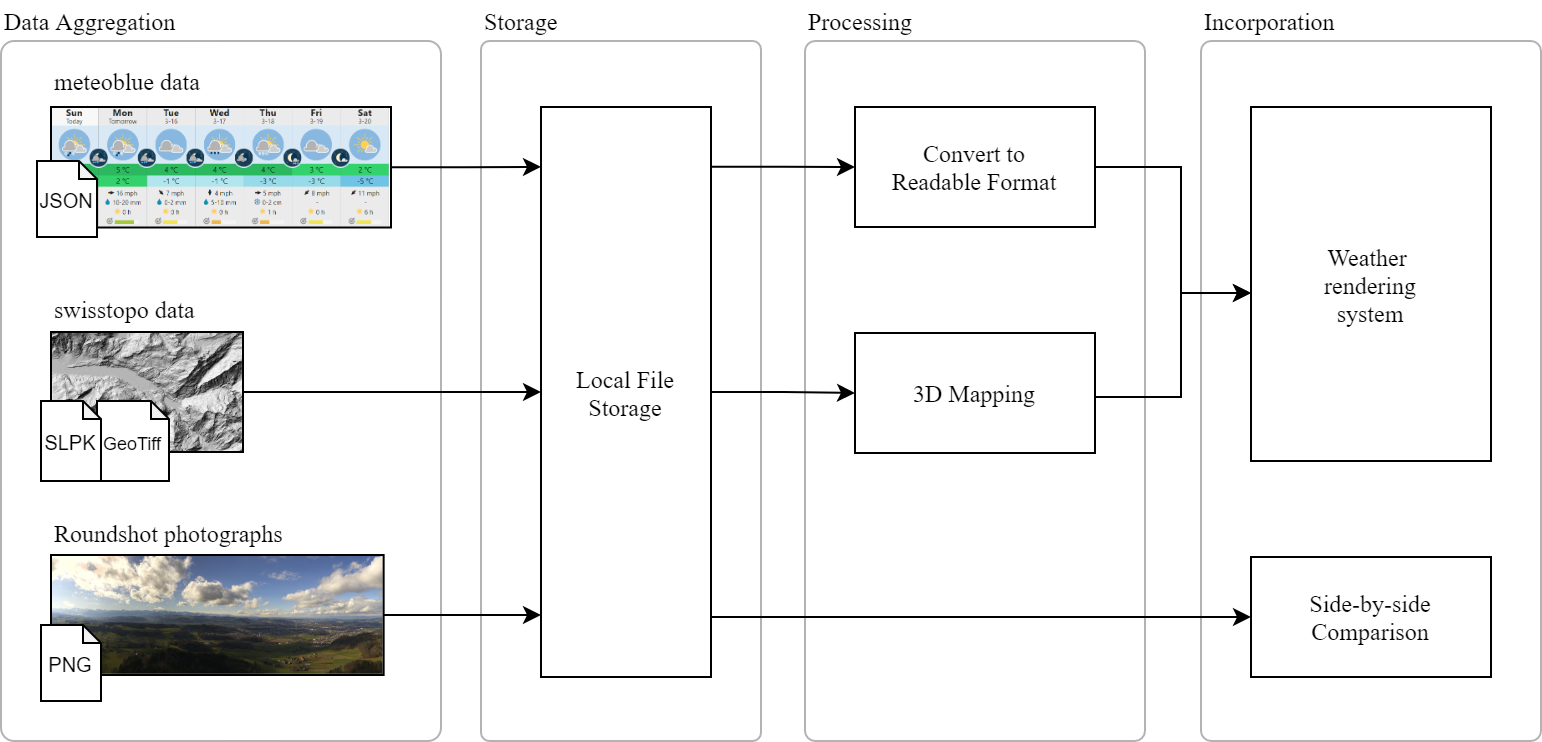
\includegraphics[width=\linewidth]{system diagram.png}
    \caption{The system overview diagram.}
    \label{img:techimpl:system}
\end{figure}

\subsection{Unity Project Architecture}
The project architecture in Unity consists of a set of \gls{volumetric} \gls{shader}s, the \emph{ArcGIS} component and some auxiliary objects.
\\
\begin{wrapfigure}[10]{r}{4cm}
    \vspace{-\baselineskip}
    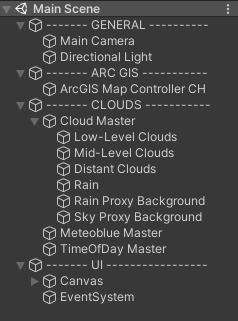
\includegraphics[width=4cm]{unity scene hierarchy.png}
    \caption{Hierarchy of the Unity project.}
    \label{img:techimpl:hierarchy}
\end{wrapfigure}
\autoref{img:techimpl:hierarchy} shows the content of the Unity scene file.
The first section, named "general", contains the standard game objects for the primary camera and for the directional lighting.
\\
The \emph{ArcGIS} component only requires a single game object, which has been placed into its own section.
\\
It is followed by the core of the weather rendering system, which is housed under the section named "clouds".
In it, there are several controlling game objects like the "meteoblue master", which are responsible for setting up the shaders.
\\
At last, the "UI" section contains the default game objects for a \gls{ui} in Unity, adjusted to this project.

\subsubsection{Scene Anatomy}
The scene setup is similar to what was originally planned. There are multiple layers of clouds, each rendered by a unique \gls{volumetric} \gls{shader}.
However, there is no layer for high-level clouds. It turned out that the intricate visual appearance of cirrus clouds was more difficult to simulate than anticipated.
\\
The current scene anatomy is depicted in the following graphics, as viewed from the side.


\begin{figure}[H]
    \centering
    \begin{tikzpicture}[scale=1]
        \tikzset{edge/.style = {-{Latex[length=3mm]},shorten >= -4pt}}
        \tikzset{shortedge/.style = {shorten <=-4pt,shorten >= -4pt}}
        \tikzset{icon/.style = {font=\Large}}
        \tikzset{mini/.style = {font=\footnotesize}}
        \tikzset{tiny/.style = {font=\tiny}}

        % cloud layer boxes
        \node[inner sep=0pt] at (6,4) 
            {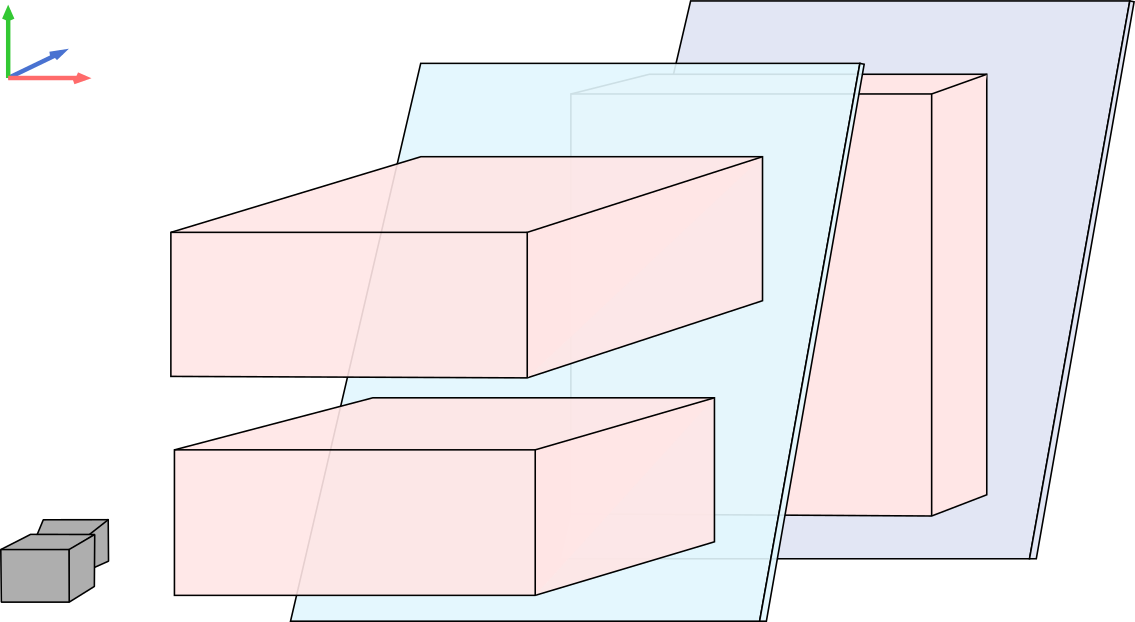
\includegraphics[width=0.8\textwidth]{anatomy.png}};

        \node at (0.3,0.5) {camera};

        % labels
        \node[red] at (2.3,2.1) {$C_{low}$};
        \node[red] at (2.3,4.5) {$C_{mid}$};
        \node[red] at (9.3,2.2) {$C_{back}$};
        \node[darkercyan] at (5.00,6.40) {$P_{rain}$};
        \node[darkercyan] at (7.85,7.05) {$P_{sky}$};
        \node[tiny] at (00.95,6.52) {$x$};
        \node[tiny] at (-0.06,7.45) {$y$};
        \node[tiny] at (00.65,6.90) {$z$};
        
    \end{tikzpicture}
    \captionof{figure}{Compute shader thread group with labeled dimensions.}
    \label{img:tikz:techimpl:anatomy}
\end{figure}


\subsection{Meteoblue Integration}
\label{section:techimpl:meteoblue}
While the bachelor project specifictation document described the use of \emph{meteoblue}'s "basic 1h" package, this was not the only package that was used in the final implementation.
After the cancellation of the technical interview with \emph{meteoblue} and further research into additional, available weather data sources, the package "clouds 1h" was suggested.
It provides an overview of cloud coverage percentage for each cloud layer, which is exactly what the implementation was missing.
\emptyline
\begin{tabularx}{\linewidth}{|l|X|}
    \hline
    \textbf{Package name}   & \textbf{Description} \\ \hline
    Basic (1h)              & Mainly used for shading and visual effects. \\ \hline
    Clouds (1h)             & Mainly used for cloud coverage data. \\ \hline
\end{tabularx}
\emptyline
The following table displays a list of properties from both data packages and how they are used in the final implementation.
\emptyline
\begin{tabularx}{\linewidth}{|l|l|X|}
    \hline
    \textbf{Property name}      & \textbf{Source}     & \textbf{Usage}                                 \\ \hline
    Wind speed                  & Basic (1h)          & Used with a multiplier                         \\ \hline
    Wind direction              & Basic (1h)          & Converted form degrees to a directional vector \\ \hline
    Precipitation               & Basic (1h)          & Used for controlling rain particle system and cloud color.\newline Factored into cloud edge highlight colors from sunshine.\newline Factored into skybox colors. \\ \hline
    Precipitation probability   & Basic (1h)          & Included in approximation of precipitation     \\ \hline
    Cloud coverage low          & Clouds (1h)         & Used for the weather in Bern                   \\ \hline
    Cloud coverage mid          & Clouds (1h)         & Used for the weather in Bern                   \\ \hline
    Cloud coverage high         & Clouds (1h)         & Used for the weather in Bern                   \\ \hline
    Total cloud coverage        & Clouds (1h)         & Used for the distant weather                   \\ \hline
\end{tabularx}
\emptyline
Other properties like temperature and UV index provide insufficient or irrelevant information and have therefore not been mapped.

\clearpage

\subsection{ArcGIS Integration}
\label{section:techimpl:arcgis}
During the research phase of the project, the \emph{ArcGIS Maps SDK for Unity} \cite{arcgis:unitysdk} was found. This proved to be a suitable replacement for the originally planned \emph{swisstopo} elevation model data.
The plugin was easily installed. The setup process required minimal amount of effort and the plugin was ready to run in no time. 

\begin{figure}[H]
    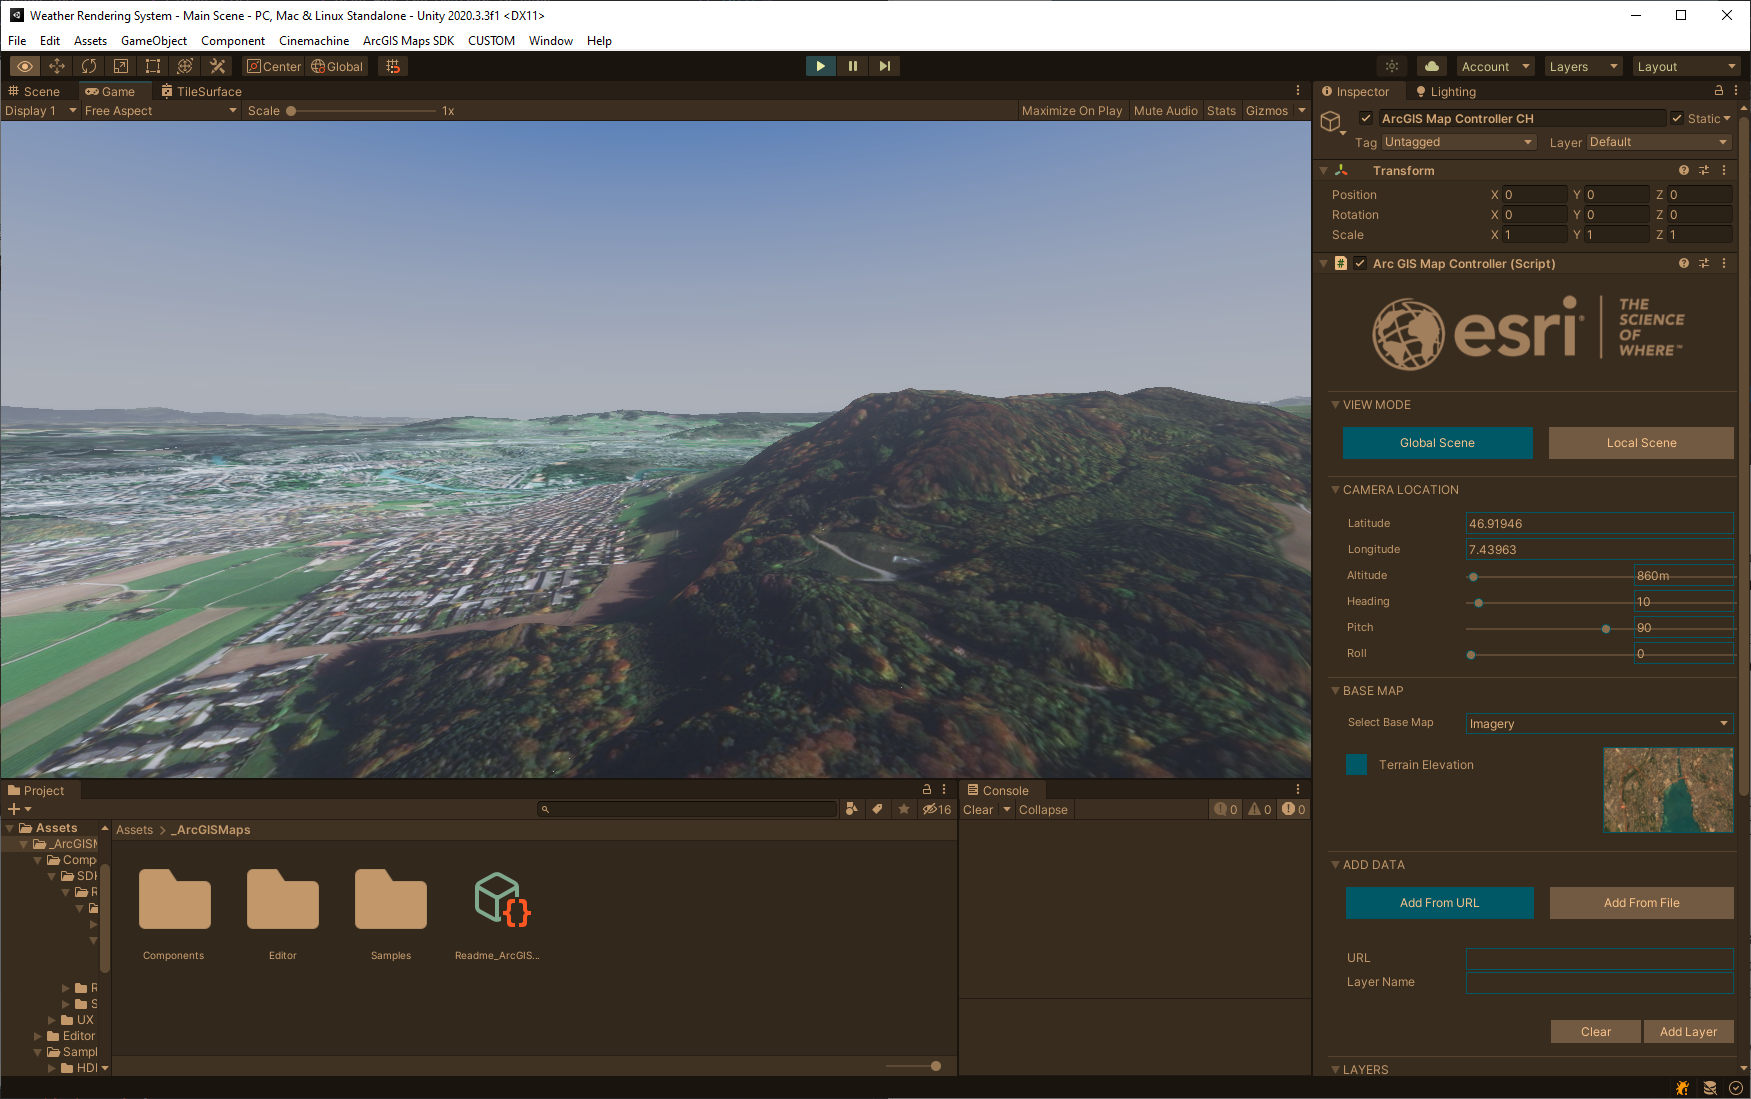
\includegraphics[width=\linewidth]{unity-sdk2.png}
    \caption{ArcGIS Maps SDK for Unity \protect\cite{arcgis:unitysdk}.}
\end{figure}

\noindent
The plugin generates and renders map tiles according to the elevation model and automatically maps aerial photographs as textures on top.
This happens during runtime and is continuously updated.
\\
After setting up the plugin in Unity, the camera needed to be positioned on top of the Gurten mountain. Also, there needed to be a translation mechanic to move the camera to the top of the Bantiger mountain.
This was done with via script and is not part of the \emph{ArcGIS} plugin.

\subsection{Shader Architecture}
\label{section:techimpl:architecture}
The architecture described in the implementation approach in \sectionref{section:impl:layers} was chosen, but underwent some alterations.
First, 
TODO
TODO
TODO
TODO
TODO
TODO

\subsection{Noise Generation}
\label{section:techimpl:noise}
As extensively described in \sectionref{section:noise}, the \gls{noise} texture is generated by a \gls{computeshader}.
The resulting 3D texture is seamless and is solely based on the Voronoi \gls{noisegeneration} algorithm, invoked with different scales and octaves.
In the final texture, each \gls{texel} holds four different \gls{noise} values, one for each color channel.
\\
The compute shader is dispatched only once, at the start of the simulation. This saves on a great deal of performance, as the \gls{noise} does not need to be recalculated each frame.

\subsection{Shadow Casting}
\label{section:techimpl:shadow}
The \gls{volumetric} cloud \gls{shader}s do not contain a \gls{shadowpass}, which means that the cloud objects do not cast any shadows.
The reason for this is that the \emph{ArcGIS} plugin generates and renders the 

\subsection{Results}
\label{section:techimpl:results}

\subsection{Testing}
\label{section:techimpl:testing}

\subsection{Measurability}
\label{section:techimpl:measure}

\subsection{Comparison to Implementation Approach}
\label{section:techimpl:comparison_impl}

\subsection{Comparison to Previous Work}
\label{section:techimpl:comparison}
%performance

2. technical impl: algorithms, progress pics, 
2. results: what has been achieved, how realistic, compare to spec
2. testing: 1-2 paragraphs, visual testing, gui stuff, messbarkeit,
